%% IEEE Transactions on Information Theory -- single-column review manuscript.
%% Author: Andrew H. Bond, Senior Member, IEEE. Generated for submission via the
%% IEEE Author Portal (https://ieee.atyponrex.com/journal/t-it). Single column is
%% the required review format; final accepted version converts to two-column.
\documentclass[journal,onecolumn,11pt]{IEEEtran}
\usepackage[T1]{fontenc}
\usepackage[utf8]{inputenc}
\usepackage{amsmath,amssymb,amsthm}
\usepackage{booktabs}
\usepackage{array}
\usepackage{xcolor}
\usepackage{tikz}
\usetikzlibrary{arrows.meta,positioning,calc,fit,backgrounds}
\usepackage{pgfplots}
\pgfplotsset{compat=1.17}
\usepackage[colorlinks=true,linkcolor=blue,citecolor=blue,urlcolor=blue]{hyperref}

\newtheorem{theorem}{Theorem}
\newtheorem{proposition}{Proposition}
\newtheorem{lemma}{Lemma}
\newtheorem{definition}{Definition}
\newtheorem{corollary}{Corollary}
\theoremstyle{remark}
\newtheorem*{remark}{Remark}

\newcommand{\PC}{P_{\mathcal{C}}}
\newcommand{\Sd}{\Sigma_{\delta}}
\newcommand{\tr}{\operatorname{tr}}
\newcommand{\dO}{d_{\mathcal{O}}}
\newcommand{\E}{\mathbb{E}}
\newcommand{\R}{\mathbb{R}}

\begin{document}

\title{Observation Theory: Geometry, Distortion, and\\ Reliability as Properties of Observation}

\author{Andrew~H.~Bond,~\IEEEmembership{Senior~Member,~IEEE}%
\thanks{Manuscript submitted July 2026. The author is with the Department of
Computer Engineering, San Jos\'e State University, San Jos\'e, CA 95192 USA
(e-mail: andrew.bond@sjsu.edu; ORCID 0009-0003-2599-6158).}%
\thanks{Companion software, the sealed pre-registrations, and the claim ledger that
govern every empirical result are publicly available at
\url{https://github.com/ahb-sjsu/geometric-observation}. A continuous-integration
workflow re-runs the reproducible experiments and verifies the theoretical
constructions on each commit.}}

\markboth{IEEE TRANSACTIONS ON INFORMATION THEORY (SUBMITTED)}%
{BOND: OBSERVATION THEORY}

\maketitle

\begin{abstract}
We develop Observation Theory, the thesis that operational geometry, distortion, and
reliability are properties not of an object alone but of the relation among the
object, an observer, a channel, and a resolution budget. An observer is a consumer, a
map from a representation to a task output, with a metric on that output. A
second-order expansion of the downstream distortion isolates one controlling quantity:
the reconstruction error read through the consumer, the trace of the error second
moment weighted by a positive semidefinite read operator, the pullback of the output
metric along the consumer. Ordinary reconstruction is the isotropic corner where this
operator is the identity, the home of the Gaussian mean squared error specialization
of Shannon rate distortion and of Gauss least squares. We prove that the read operator
is the pullback geometry of distinguishability, inducing a quotient of the
representation by what the consumer cannot separate; that it is recoverable from black
box consumer queries under a specified observation distribution; and that it defines a
consumer relative rate distortion function whose achievability and converse we
establish for a general source, with a coding theorem for the true nonlinear consumer
divergence that reduces exactly to output coding. We instantiate the read operator for
attention, gradient optimization, and retrieval, and position it as the
identifiable geometric middle term between Shannon rate distortion and the information
bottleneck. Every empirical claim is governed by a sealed prior registration with a
preset bar; four predictions are confirmed and one is refuted.
\end{abstract}

\medskip\noindent\textbf{Index Terms---}
Rate--distortion theory, source coding, quantization, information geometry,
distinguishability, indirect source coding, information bottleneck, neural network
compression, reproducibility.


\IEEEpeerreviewmaketitle

\noindent\emph{Andrew H. Bond, Senior Member, IEEE. Department of Computer Engineering, San Jos\'e State University, San Jos\'e, CA 95192 USA. Email: andrew.bond@sjsu.edu. ORCID: 0009-0003-2599-6158.}


\section{Introduction}

Shannon fixed a distortion measure and asked for the fewest bits meeting it
\cite{shannon1948,shannon1959}; Gauss fixed the same measure and asked for the
least-squares estimate \cite{gauss1809}. This paper reads their common assumption
as the variable of interest: the error that matters is not the one a code makes but
the one a consumer \emph{reads}, and different consumers read different subspaces of
the same error. Once the distortion is that of the task, Euclidean reconstruction is one
corner---the isotropic observer $\PC=I$---and any anisotropic or rank-deficient $\PC$
reads the error differently.

The idea that one should code a source to serve a \emph{functional} of it, not the
source, is not new: it is the indirect (remote) rate--distortion problem
\cite{dobrushin1962,wolfziv1970,witsenhausen1980}; its lossless, discrete form is
coding for computing and graph entropy \cite{korner1973,orlitsky2001}; its modern
face is the rate--distortion--perception tradeoff \cite{blau2019} and task-oriented
/ semantic communication \cite{gunduz2023}; and its deployed form, for neural
networks, is loss-aware (Hessian-weighted) compression, from Optimal Brain
Damage/Surgeon \cite{lecun1990,hassibi1993} to Hessian-aware quantization and GPTQ
\cite{dong2019hawq,frantar2023gptq}. What is missing across these is a single,
\emph{identifiable geometric} object that names the task's metric and lets one
predict, recover, and test it. Observation Theory supplies it: the read operator
$\PC$, the consumer's local output metric, sitting as the geometric middle term
between Shannon's Gaussian Euclidean-MSE specialization ($\PC=I$) and the information
bottleneck \cite{tishby1999} (an arbitrary, non-geometric relevance variable). We
contribute (i) the map placing these literatures on one axis; (ii) $\PC$'s
\emph{identifiability}---recovery from black-box consumer queries under a specified
observation distribution, validated blind against a
planted ground truth, which the quantization literature (estimating the Hessian from
calibration data) never validates against truth; (iii) an ex-ante extreme-value
reliability certificate; (iv) budget-relativity of the verdict; and (v) a
registration-first empirical program---sealed predictions, ex-ante bars, a refuted
prediction reported as prominently as the confirmations---whose recurring
demonstration is a single code whose downstream verdict \emph{inverts} when nothing
changes but the consumer.
The three companion works are Paper~I (the angular observer and the spectral
budget-inversion mechanism) \cite{paper1}, Paper~II (geometric key quantization and
the reconstruction-is-not-the-target negative) \cite{paper2}, and the claim ledger
\cite{ledger2026}; this is their information-theoretic synthesis.

\section{The controlling quantity}\label{sec:framework}

\begin{table}[!t]
\centering
\footnotesize
\caption{Observation Theory as the identifiable geometric middle term between two
classical extremes. The read operator $\PC$ is the axis.}
\label{tab:positioning}
\setlength{\tabcolsep}{5pt}
\begin{tabular}{@{}p{3.1cm}p{2.2cm}p{6.2cm}@{}}
\toprule
\textbf{Framework} & \textbf{$\PC$} & \textbf{Character} \\
\midrule
Shannon rate--distortion (Gaussian MSE) & $I$ (isotropic) & fixed, task-agnostic; the reconstruction corner where Gauss least squares lives \\[2pt]
\textbf{Observation Theory} & $J^\top G J$ & geometric, positive semidefinite, water-fillable, and \emph{identifiable} from the consumer \\[2pt]
Information bottleneck & --- & an arbitrary, non-geometric relevance variable \\
\bottomrule
\end{tabular}
\end{table}

\begin{definition}[Instance]
An instance is $(X,\mathcal{C},\mathcal{Q})$: a representation with vectors
$x\in\R^{d}$, a \emph{consumer} $\mathcal{C}:\R^{d}\to\R^m$ with a divergence $D_Y$
on its outputs, and a family $\mathcal{Q}$ of lossy codes producing $\hat x=x+\delta$.
The downstream distortion is the pointwise random quantity
$\dO:=D_Y(\mathcal{C}(x),\mathcal{C}(\hat x))$, measured on the consumer output, never
assumed from the ambient metric of $X$; write $\bar{\dO}:=\E[\dO]$ for its expectation
over the instance.
\end{definition}

\begin{proposition}[Consumer-projected distortion]\label{prop:main}
Let $D_Y$ be twice differentiable with $D_Y(u,u)=0$, $\nabla_v D_Y(u,v)|_{v=u}=0$,
and \emph{local output metric} $G(u)=\nabla^2_v D_Y(u,v)|_{v=u}\succeq0$ (the Fisher
information metric when $D_Y$ is the KL divergence or a kindred statistical
divergence, a generic local metric otherwise); let
$J(x)=\partial\mathcal{C}/\partial x$. For error $\delta=\hat x-x$ with conditional
\emph{second moment} $\Sd(x)=\E[\delta\delta^\top\mid x]$, the leading-order expected
distortion is
\[
\bar{\dO} \;=\; \tfrac12\,\E_x\tr\!\big(\PC(x)\,\Sd(x)\big)\;+\;r,
\qquad \PC(x)=J(x)^\top G(\mathcal{C}(x))\,J(x)\succeq0 ,
\]
so $\PC$ is the pullback of the local output metric $G$ along $\mathcal{C}$. Making
the asymptotics explicit: for a small-noise family $\delta_\varepsilon=\varepsilon Z$
with $\E\|Z\|^2<\infty$ and the second-order Taylor remainder dominated uniformly on a
neighborhood of the diagonal, $\bar{\dO}=\tfrac{\varepsilon^2}{2}\,\E[Z^\top\PC(X)Z]
+o(\varepsilon^2)$ (i.e.\ $r=o(\varepsilon^2)$).
When $\Sd(x)$ is uncorrelated with the point-dependent weight $\PC(x)$ this factors
as $\tfrac12\tr(\PC\Sd)$ with $\PC=\E_x[\PC(x)]$, $\Sd=\E_x[\Sd(x)]$. The controlling
object is the \emph{second} moment, not the covariance: pointwise
$\tr(\PC(x)\Sd(x))=\tr(\PC(x)\,\mathrm{Cov}[\delta\mid x])+\mu_\delta(x)^\top\PC(x)
\mu_\delta(x)$ with $\mu_\delta(x)=\E[\delta\mid x]$, then averaged over $x$, so a
biased code's offset is \emph{part} of the distortion, not averaged away---which is
why quantizer bias is first-class (\S\ref{sec:readop}). Reconstruction distortion
$\E\|\delta\|^2=\tr(\Sd)$ is the \emph{isotropic} corner $\PC=I$.
\end{proposition}
\begin{proof}
Expand $\mathcal{C}(x+\delta)=\mathcal{C}(x)+J\delta+O(\|\delta\|^2)$ and $D_Y$ to
second order about its minimum; the value and gradient terms vanish, leaving
$\tfrac12\delta^\top(J^\top GJ)\delta+o(\|\delta\|^2)$. Take $\E_x$; the factored
form requires the stated uncorrelatedness (for real quantizers both $J$ and $\Sd$
depend on $x$, so the exact object is the $x$-averaged trace).
\end{proof}

We keep $\E_x\tr(\PC(x)\Sd(x))$ as primary and use the factored $\tr(\PC\Sd)$ as the
convenience it is. (We drop the harmless $\tfrac12$.)

\subsection*{Distinguishability, and the observer's quotient}

The form $\delta^\top\PC(x)\delta=(J\delta)^\top G\,(J\delta)$ is not, at root, a
compression cost; it is a \emph{distinguishability}. It measures how far the
consumer's outputs $\mathcal{C}(x)$ and $\mathcal{C}(x{+}\delta)$ separate in the
output metric $G$, and when $G$ is the Fisher information metric of the output
distribution, $\delta^\top\PC\delta$ \emph{is} the local statistical
distinguishability (the leading KL / $\chi^2$) of those outputs. So $\PC$ is the
pullback through $\mathcal{C}$ of the geometry of distinguishability: Observation
Theory is pullback geometry.

Two consequences follow, and both recur below. First, define the global operational
equivalence $x\sim_{\mathcal{C}}x'\iff D_Y(\mathcal{C}(x),\mathcal{C}(x'))=0$
(statistical indistinguishability of the outputs). Its infinitesimal shadow is
$\ker\PC(x)=\ker\!\big(G^{1/2}J\big)$, which equals $\ker J$ when $G\succ0$ on
$\operatorname{im}J$ but is larger when $G$ is only semidefinite---the output can move
parametrically yet stay indistinguishable. Under a constant-rank / integrability
condition on $\PC(x)$ this null distribution integrates to leaves tangent to
$\ker\PC(x)$; that the \emph{global} divergence vanishes along each leaf---so the
leaves are exactly the fibers of $\sim_{\mathcal{C}}$---needs a further compatibility
condition, namely $D_Y(\mathcal{C}(x),\mathcal{C}(x'))=0$ along them (equivalently,
$\mathcal{C}$ factors through $X/\!\sim_{\mathcal{C}}$). Where it holds, the
consumer's true object is the quotient $X/\!\sim_{\mathcal{C}}$, not $X$:
perturbations in $\ker\PC$ exist in the representation but have \emph{no operational
consequence}. In the fixed-$\PC$ model of \S\ref{sec:rd} this quotient is represented
by $\Pi X$ and Prop.~\ref{prop:floor} gives the zero-distortion rate
$R_{\mathcal{C}}(0)=H(\Pi X)$; the point-dependent case is settled unconditionally in
Appendix~\ref{app:true} (Cor.~\ref{cor:B2a}: $R_{\mathcal{C}}(0)=H(\mathcal{C}(X))$,
via the true divergence, needing none of the compatibility conditions above)---rate
is expended only on distinctions the consumer can resolve. Second, $\ker\PC$ is
gauge-like \emph{but only relative to $\mathcal{C}$}: another consumer may read those
directions, so it is not a true gauge redundancy (which would be invisible to every
admissible observer). One observer's noise is another's signal; one observer's state
variable is another's gauge freedom. Adjoining the budget of \S\ref{sec:rate}, an
observer is a triple $\mathcal{O}=(\mathcal{C},G,B)$---readout, output metric, and
resolution---and the geometry it resolves is relative to all three.

\begin{quote}
\textbf{Principle of observational relativity.} Operational fidelity, distortion,
and resolved geometry are not properties of the object alone; they are properties of
the relation among object, observer $(\mathcal{C},G)$, channel, and budget, and are
ill-posed until all are specified. Observation induces geometry; each observer pulls
back a distinct operative geometry and quotient.
\end{quote}

The rest of the paper derives $\PC$ for concrete consumers, shows it recoverable
from queries, and studies what the channel (\S\ref{sec:capacity}) and budget
(\S\ref{sec:rate}) do to the geometry it induces.

\section{Derivation of the read operator}\label{sec:readop}

\begin{table}[!t]
\centering
\footnotesize
\caption{The read operator $\PC$ instantiated for three consumers. Ordinary
reconstruction is the isotropic corner $\PC=I$.}
\label{tab:readops}
\setlength{\tabcolsep}{5pt}
\begin{tabular}{@{}p{2.1cm}p{2.4cm}p{4.3cm}p{4.2cm}@{}}
\toprule
\textbf{Consumer} & \textbf{Output divergence $D_Y$} & \textbf{Read operator $\PC$} & \textbf{Recovered from} \\
\midrule
Softmax attention & Kullback--Leibler & query second moment $\E[qq^\top]$ (coupled expectation) & finite-difference Jacobian probe of the softmax output \\
Gradient optimizer & quadratic step error & Hessian $H$ (Gauss--Newton curvature if nonconvex) & calibration curvature estimate \\
Retrieval ranking & margin / rank loss & subspace projector $\E[qq^\top]$ & query-bank second moment \\
Reconstruction & squared Euclidean & identity $I$ (isotropic corner) & --- (task-agnostic) \\
\bottomrule
\end{tabular}
\end{table}

\begin{proposition}[Softmax attention]\label{prop:softmax}
Read keys $\{k_s\}_{s=1}^{S}$ through a query bank: logits $l_s=q^\top k_s/\sqrt{d}$,
output $p=\mathrm{softmax}(l)$, $D_Y=\mathrm{KL}$. Under key perturbation $\delta_s$,
\[
\bar{\dO}=\tfrac{1}{2d}\,\E_q\,\mathrm{Var}^{\,p}_s\!\big(q^\top\delta_s\big)
+O(\|\delta\|^3)
=\tfrac{1}{2d}\,\E_q\tr\!\big(qq^\top A_q\big)+O(\|\delta\|^3),
\qquad A_q=\sum_s p_s(q)\,\tilde\delta_s\tilde\delta_s^\top,
\]
where $\tilde\delta_s=\delta_s-\sum_{s'}p_{s'}\delta_{s'}$ is the across-token
$p$-demeaned error and $A_q$ its $p(q)$-weighted second moment. This
\emph{factors} to $\tfrac{1}{2d}\tr(Q\,\bar\Sigma_\delta)$, with $Q=\E_q[qq^\top]$
and $\bar\Sigma_\delta=\E_q[A_q]$, \emph{only} when $A_q$ is uncorrelated with
$qq^\top$ (the proviso of Prop.~\ref{prop:main}); in general the expectation stays
coupled, since $p$ depends on $q$.
\end{proposition}
\begin{proof}
The Fisher metric of $\mathrm{softmax}$ is $G=\mathrm{diag}(p)-pp^\top$, so
$\mathrm{KL}(p\|\mathrm{softmax}(l+\Delta l))=\tfrac12\mathrm{Var}^p_s(\Delta l_s)
+O(\Delta l^3)$ with $\Delta l_s=q^\top\delta_s/\sqrt d$. The $-pp^\top$ term is the
softmax's invariance to a common logit shift; it removes the $p$-mean, giving
$\tilde\delta_s$. Since $p$ depends on $q$, the outer $\bar\Sigma_\delta$ carries the
$\E_q$ and the final $Q$-factorization inherits the uncorrelatedness proviso of
Prop.~\ref{prop:main}.
\end{proof}
Two consequences are the phenomena we later measure. The feature-space factor is
generated by $qq^\top$, reducing to $Q=\E_q[qq^\top]$ under the decorrelation /
uniform-weight regime above; so an isotropic bank yields an isotropic feature
operator (reconstruction-like) while a subspace bank projects---the read operator,
hence the winning code, changes with the query distribution. And only the
\emph{demeaned} error survives, so the across-token mean is a nuisance the softmax
cannot see. This last fact resolves an apparent tension with the DC-offset
collapse of Paper~II \cite{paper2}: a truly common error component is free by shift
invariance, but a per-channel DC \emph{offset} is not a common component---it inflates
the quantizer's range, wasting levels and enlarging the \emph{visible} per-token
error, which is exactly why an asymmetric zero-point (asym-NF4) repairs it at no bit
cost. Invisible-to-the-consumer and free-to-encode are the same statement; range
waste is a different one.

\begin{proposition}[Gradient-descent optimizer; exact]\label{prop:opt}
Let $L(\theta)=\tfrac12\theta^\top H\theta$ with $H\succeq0$, $g=H\theta$, and
$\hat g=g+\delta$ with conditionally unbiased error $\E[\delta\mid\theta]=0$, used in
a step of size $\eta$. Then $L(\theta-\eta\hat g)-L(\theta-\eta g)=\tfrac12\eta^2\,
\delta^\top H\delta-\eta\,\delta^\top H(\theta-\eta g)$, whose error-quadratic part
is $\tfrac12\eta^2\tr(H\,\delta\delta^\top)$; the linear cross term vanishes in
expectation ($\E[\delta\mid\theta]=0$), giving $\E[\dO]=\tfrac12\eta^2\tr(H\,\Sd)$,
so $\PC=H\succeq0$ \emph{exactly}.
\end{proposition}
\noindent This is loss-aware pruning/quantization made a metric: Hessian-weighted
deletion \cite{lecun1990,hassibi1993,dong2019hawq,frantar2023gptq} \emph{is}
$\tr(H\Sd)$, and calibration-based Hessian estimation is the production form of the
probe of \S\ref{sec:id}. Reconstruction is the flat case $H=I$. For a non-convex
loss the Hessian may be indefinite; the metric reading then takes $\PC$ to be the
PSD Gauss--Newton / Fisher curvature in place of $H$.

\begin{remark}[Retrieval]
For score-ranking $s(q,x_i)=q^\top x_i$, the inverted-pair fraction is, to leading
order for smooth rank statistics, monotone in
$\tr(\PC\bar\Sigma_\delta)/\tr(\PC\bar\Sigma_0)$, with $\PC=\E[qq^\top]$,
$\bar\Sigma_\delta=\mathrm{Cov}_i(\delta_i)$ the across-item error covariance and
$\bar\Sigma_0=\mathrm{Cov}_i(x_i)$ the signal covariance (both demeaned across items);
$\PC$ is a subspace projector when queries concentrate. Rank statistics are
non-smooth; we treat this instance empirically (\S\ref{sec:distortion}).
\end{remark}

\section{Distortion: the consumer determines the metric (GO-2)}\label{sec:distortion}

\begin{figure}[!t]
\centering
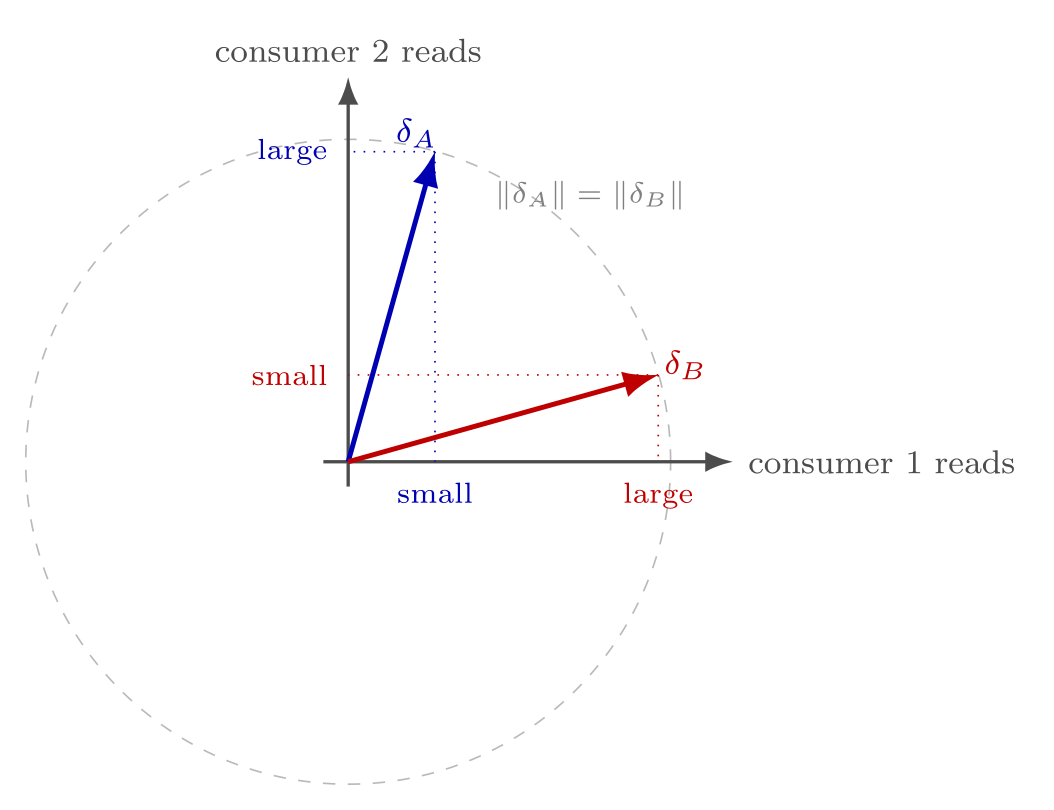
\includegraphics[width=0.62\linewidth]{fig1_flip.png}
\caption{The flip. Two lossy codes produce errors $\delta_A,\delta_B$ of \emph{equal}
reconstruction norm (dashed circle), so reconstruction cannot separate them. Consumer~1
(horizontal read operator) sees a small $\delta_A$ projection and a large $\delta_B$
one, and prefers code~$A$; consumer~2 (vertical read) prefers code~$B$. The downstream
verdict $\tr(\PC\Sigma_\delta)$ reverses with the read operator while reconstruction
remains blind---the characteristic signature of Observation Theory.}
\label{fig:flip}
\end{figure}

Proposition~\ref{prop:softmax} predicts that at matched reconstruction the ranking of
two codes is set by $\tr(\PC\Sd)$, hence by the query distribution.

\paragraph{Dissociation.} Two 4-bit codes at an audited matched budget (spread
$0.19$ bit) with \emph{identical} reconstruction ($0.0938$ vs $0.0934$): the
whole-vector code is $2.53\times$ worse on softmax-KL ($12/12$ seeds); a
wrong-quotient control is $21\times$ worse at $\sim\!5\times$ the reconstruction.
Reconstruction is not the controlling quantity (\texttt{[demonstrated]}).

\paragraph{Flip.} Holding reconstruction fixed and changing only the query bank, the
ranking \emph{inverts}: isotropic $\Rightarrow$ code $a$ better ($2.5\times$,
$12/12$); subspace $\Rightarrow$ code $b$ better ($12/12$). The directly computed
$\tr(\PC\Sd)$ tracks the sign on every seed in both consumers; reconstruction, a
consumer-blind scalar, cannot (rank correlation $0.40$ vs $1.00$). This is
Proposition~\ref{prop:softmax} with $Q$ swapped (\texttt{[demonstrated]}).

\paragraph{Replication and out-of-sample.} The flip replicates on retrieval ranking
(different representation, set-valued consumer): identical reconstruction
($0.0964$), ranking flips with the read subspace (log-advantage $-4.70$ vs $+4.65$,
$12/12$), $\tr(\PC\Sd)$ tracking, reconstruction blind (\texttt{[replicated]}). It
generalizes to optimization with $\PC=H$ (Prop.~\ref{prop:opt}): at matched
reconstruction the curvature-metric distortion flips between two Hessians ($12/12$),
tracked by $\tr(H\Sd)$, reconstruction uninformative ($-0.20$)---and under $H=I$
reconstruction tracks \emph{perfectly} ($1.00$), the derived $\PC=I$ corner observed
(\texttt{[predicted]}, out-of-sample). One derivation; three read operators. These
consumers are \emph{synthetic}---the point is to validate the theory's logic (the
$H=I$ positive control being the clean confirmation); the trained-model hardening
(\S\ref{sec:discussion}), attempted prospectively, initially missed on a
non-reconstruction-matched design and is then \emph{cleared} by a corrected,
reconstruction-matched rematch on a real Llama attention layer.

\section{Identifiability: the read subspace is recoverable (GO-1)}\label{sec:id}

\begin{proposition}[Recovery of the read subspace]\label{prop:id}
Let $\mathcal{C}(x)=f(Wx)$, $W\in\R^{r\times d}$ of rank $r$, $f$ coordinatewise with
$\E[f_i'(Wx)^2]>0$ for every coordinate $i$ (no saturated unit). Then
$\E_x[J^\top J]=W^\top\E[\mathrm{diag}(f'^2)]W$ has rank $r$ with column space
$\operatorname{row}(W)$, so its top-$r$ eigenvectors span the read subspace; a
finite-difference estimate $\hat J u\approx(\mathcal{C}(x{+}hu)-\mathcal{C}(x{-}hu))/2h$
recovers it from consumer queries alone.
\end{proposition}

We built such a probe---receiving only the callable $\mathcal{C}(\cdot)$ and the
dimensions, never $W$, the codes, or $\dO$ (blinding enforced in code). It recovers
the planted read subspace at overlap $0.936$ against a $0.059$ chance baseline
($\approx16\times$), and the \emph{blind} $\tr(\hat\PC\Sd)$ predicts the flip of
\S\ref{sec:distortion} on $12/12$ seeds in both consumers with rank correlation
$1.00$---identical to ground truth---while reconstruction cannot ($0.40$)
(\texttt{[predicted]}). Two scope notes. Prop.~\ref{prop:id} recovers the read \emph{subspace} for the
$f(Wx)$ model with a Euclidean output metric; recovering the \emph{full} operator
$\E_x[J^\top G J]$---its eigenvalues, and a general $G$---is the broader program.
And $\PC$ depends on the probe-point distribution and on $G$, so it is identifiable
from black-box consumer queries \emph{under a specified observation distribution},
not from the callable alone. Loss-aware compression estimates such a metric from
calibration data; the contribution here is validating \emph{recovery against a
planted ground truth under enforced blinding}, and composing it: from consumer
queries under that distribution one predicts which code wins, before compressing
anything.

\section{Capacity: a derived vacuity threshold (GO-3)}\label{sec:capacity}

\begin{figure}[!t]
\centering
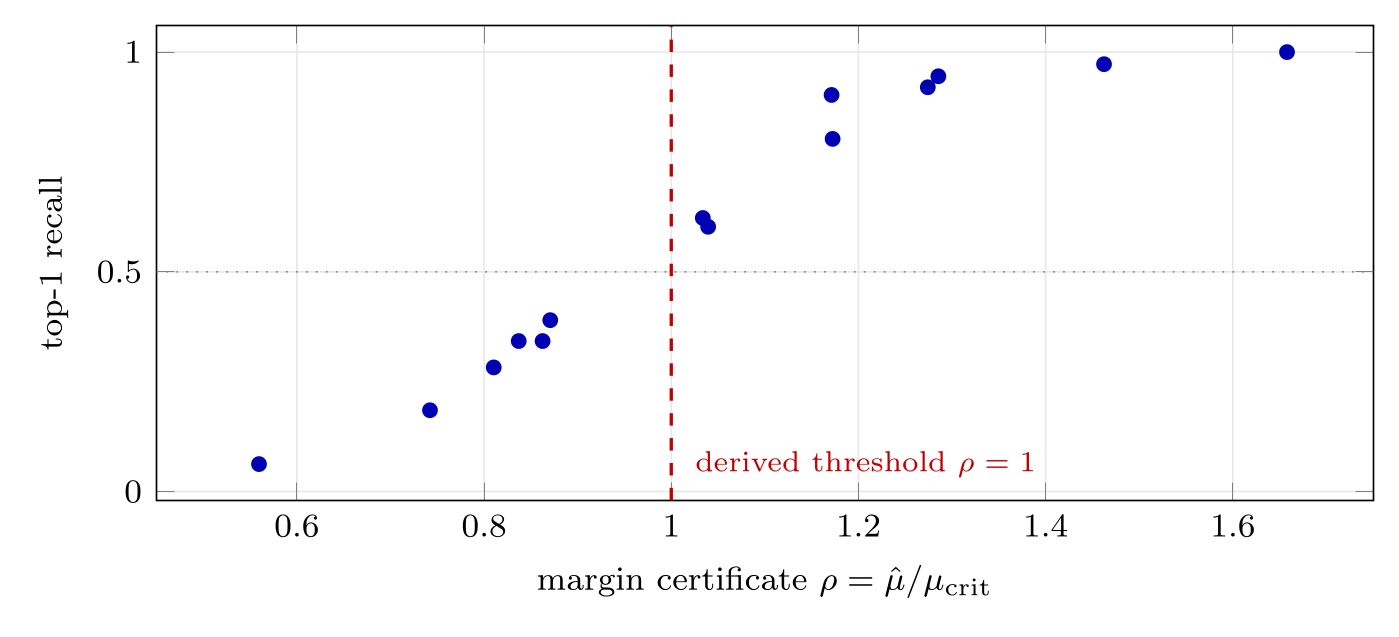
\includegraphics[width=0.85\linewidth]{fig2_vacuity.png}
\caption{Capacity (GO-3), from the committed result artifact. The derived margin
certificate $\rho$ orders top-1 retrieval recall across $14$ structurally distinct
corpora at Spearman correlation $0.99$; the recall-$\tfrac12$ crossing sits at
$\rho\approx0.95$, near the extreme-value vacuity threshold $\rho=1$ (dashed) at which
the channel is predicted to die \emph{before} any retrieval is run.}
\label{fig:vacuity}
\end{figure}

\begin{proposition}[Retrieval vacuity threshold]\label{prop:capacity}
Model the $N\!-\!1$ distractor scores, standardized to mean $0$, variance $1$, as
i.i.d.\ standard Gaussian (a reference model). Since $\Pr[M_{N-1}\le m]=\Phi(m)^{N-1}$,
top-1 success $\Pr[\hat\mu>M_{N-1}]$ crosses $\tfrac12$ at the \emph{exact median}
of the maximum,
\[
\mu_{\mathrm{crit}}:=\operatorname{med}(M_{N-1})=\Phi^{-1}\!\big(2^{-1/(N-1)}\big),
\qquad \text{leading asymptotic }\sqrt{2\ln(N{-}1)},
\]
where $\hat\mu=(\overline{\text{true}}-\overline{\text{distr}})/\mathrm{std}$ is the
margin certificate and $\rho=\hat\mu/\mu_{\mathrm{crit}}$; the certificate is
\emph{vacuous} for $\rho<1$.
\end{proposition}
\begin{proof}[Derivation]
$\Pr[M_{N-1}\le m]=\Phi(m)^{N-1}$; setting it to $\tfrac12$ gives $m=\Phi^{-1}(2^{-1/(N-1)})$,
the exact median. The Gumbel centering is $\alpha_N=\sqrt{2\ln(N{-}1)}-b_N(\ln\ln(N{-}1)
+\ln4\pi)/2$ with scale $b_N=1/\sqrt{2\ln(N{-}1)}$; the crude $\sqrt{2\ln(N{-}1)}$
omits the $-b_N(\ln\ln(N{-}1)+\ln4\pi)/2$ correction and so \emph{overshoots}. Median
and mean share this centering and differ at order $b_N$:
$\operatorname{med}(M_{N-1})=\alpha_N-b_N\ln\ln2+o(b_N)$ and
$\E[M_{N-1}]=\alpha_N+\gamma b_N+o(b_N)$ ($\gamma$ Euler--Mascheroni), so the mean
exceeds the median by $(\gamma+\ln\ln2)\,b_N$. The recall-$\tfrac12$ crossing is the
exact median $\Phi^{-1}(2^{-1/(N-1)})$---not the mean, not the leading order.
\end{proof}

Across $14$ structurally distinct corpora the certificate orders them by recall at
rank correlation $0.991$, beating the un-normalized margin ($0.873$), with a
finite-width transition (\texttt{[demonstrated]}). The registered harness used the
\emph{mean} $\E[M_{N-1}]$ (Monte-Carlo) as its $\mu_{\mathrm{crit}}$ reference, and
the recall-$\tfrac12$ crossing sits at $\rho=0.948$---slightly \emph{below} $1$
against that reference. This is expected and quantitative: the exact $\tfrac12$
threshold is the \emph{median}, below the mean by $\Theta(1/a_N)$, so the $\sim\!5\%$
shortfall is largely the mean--median offset (against the exact median of this
proposition the crossing sits at $\approx1$). Positive dependence among distractors
\emph{can} lower it further by reducing the effective count; heavier tails, by
contrast, \emph{raise} the maximum---the two must not be grouped. The exact
$\tfrac12$ crossing further assumes a \emph{fixed} standardized true margin and
i.i.d.\ Gaussian distractors; when the true score is itself random or correlated with
the distractors, $\rho$ is a reference certificate rather than an exact recall
threshold. The \emph{form} of the threshold is nonetheless robust: the
$\sqrt{2\ln N}$ scaling is the centering of the Gumbel max-domain of attraction,
shared by every distractor law with sub-exponential (lighter-than-polynomial)
tails---Gaussian, exponential, Weibull-type---so non-Gaussianity \emph{within} that
domain moves the constants $(\alpha_N,b_N)$, not the scaling law; positive correlation
enters as an \emph{effective count}, replacing $N$ by $\theta N$ through the extremal
index $\theta\in(0,1]$ and shifting $\mu_{\mathrm{crit}}$ by
$\tfrac{\ln\theta}{2\sqrt{2\ln N}}$ at leading order; and only genuinely heavy
(Fr\'echet-domain, polynomial) tails change the scaling itself---the certificate's
stated failure mode. The $14$-corpus ordering above ($\rho=0.99$ on clustered,
non-Gaussian real embeddings) is the empirical counterpart: real structure shifts the
absolute death point but preserves the ordering the certificate is used for.
Capacity says, from a computable quantity, \emph{where} the channel dies
before any retrieval is run.

\section{Rate: the operative verdict depends on the budget (GO-4)}\label{sec:rate}

The read operator, capacity, and distortion are stated at a fixed observer budget;
the budget is a rate, and it inverts the verdict. The mechanism is spectral: an
eigenfunction $\varphi_k$ with eigenvalue $\lambda_k$ oscillates on the wavelength
$\lambda_k^{-1/2}$, and Weyl's law $N(\lambda)\sim c\,\mathrm{Vol}(M)\lambda^{d_M/2}$
($d_M$ the intrinsic dimension) grows the count of modes below a fixed scale with
resolution.

\begin{lemma}[Fixed-band consistency]\label{lem:band}
At a fixed low-mode budget $m$, as the sample grows the graph operator converges
spectrally to the manifold operator \cite{calder2022}, so the fixed low-$\lambda$
band sharpens and geodesic fidelity \emph{converges toward its continuum value} and is
predicted to improve asymptotically (the spectral-convergence mechanism of
Paper~I \cite{paper1}). Convergence does not force step-wise monotonicity in $N$; the
monotone finite-sample trend below is the \emph{registered empirical} result, not a
consequence of the lemma.
\end{lemma}

Holding instead the resolved scale $\tau$ fixed (spectral-gap matching), $m=N(\tau)$
grows with $N$; the newly resolved modes near $\tau$ have wavelength approaching the
sampling scale and, for a non-ideal substrate, inject sub-geodesic detail, so
geodesic fidelity is nonincreasing---Paper~I's registered inversion \cite{paper1}. We
replicate it on a new substrate: $768$-dimensional multilingual book-paragraph
embeddings (Project Gutenberg translations; $32{,}000$ points, three seeds). Fixed
$m=10$: geometry preservation rises with $N$ (trend $+0.4,+1.0,+1.0$).
Spectral-gap-matched, $m:10\to121/126/159$: geometry \emph{collapses} (trend $-1.0$
every seed); the budgets agree at the smallest $N$ (gap $\le0.002$)
(\texttt{[replicated]}). Opposite verdicts about the same data, set by the observer's
rate: ``clean geometry'' is a relation between observer resolution and substrate
scale, not a substrate invariant.

\section{A consumer-relative rate--distortion function}\label{sec:rd}

The consumer-projected distortion is the single-letter measure
$d_{\mathcal{C}}(x,\hat x)=(x-\hat x)^\top\PC(x-\hat x)$ for a \emph{fixed} $\PC$
(constant, or the average $\E_x[\PC(x)]$ under the proviso of Prop.~\ref{prop:main});
define $R_{\mathcal{C}}(D)=\inf\{I(X;\hat X):\E\,d_{\mathcal{C}}(X,\hat X)\le D\}$.
This fixed-$\PC$ model must be kept distinct from the \emph{local} observation metric
$\PC(x)$ of Prop.~\ref{prop:main}: for a nonlinear consumer $\PC(x)$ varies, there is
no single tilted source---a direction invisible at one point can be visible at
another---and the coding theorem for that case is open. The results below, and
Appendix~\ref{app:coding}, are for the fixed weighted-quadratic model, whose theory
is classical \cite{berger1971}.

\begin{proposition}[Gaussian rate--distortion; Berger reduction]\label{prop:rd}
For $X\sim\mathcal{N}(0,\Sigma_x)$, in the basis diagonalizing
$\PC^{1/2}\Sigma_x\PC^{1/2}$ with eigenvalues $\gamma_i$,
\[
R_{\mathcal{C}}(D)=\sum_i \tfrac12\log_2^{+}\!\frac{\gamma_i}{\theta},\qquad
\sum_i\min(\gamma_i,\theta)=D,
\]
a reverse water-filling on the $\PC$-weighted source spectrum. For $\PC=I$ this is
Shannon's Gaussian $R(D)$ \cite{shannon1959}; the estimation dual is Gauss--Markov
least squares \cite{gauss1809}.
\end{proposition}
\begin{proof}
$\tr(\PC\Sd)=\|\PC^{1/2}(x-\hat x)\|^2$; with $y=\PC^{1/2}x$ this is MSE on
$y\sim\mathcal{N}(0,\PC^{1/2}\Sigma_x\PC^{1/2})$, and Shannon water-filling applies.
The transform is invertible off $\ker\PC$, on which the consumer is blind and no rate
is spent.
\end{proof}

Bits water-fill on directions the consumer reads \emph{and} the source varies,
spending nothing on $\ker\PC$---why a reconstruction-optimal code ($\PC=I$
allocation) is beaten by a consumer-matched one when $\PC\ne I$, and why the winner
\emph{flips} with $\PC$ (\S\ref{sec:distortion}). The $H=I$ control confirms it: only
at the isotropic $\PC=I$ is reconstruction the right objective, and there it is
exactly right.

\begin{proposition}[Consumer-lossless floor; discrete source]\label{prop:floor}
Let $X$ be discrete with finite entropy, $\Pi$ the projector onto
$\operatorname{range}(\PC)$. There exist codes with $\tr(\PC\Sd)=0$ at rate
\[
R_{\mathcal{C}}(0)=H(\Pi X)\le H(X),\qquad H(X)-R_{\mathcal{C}}(0)=H(X\mid\Pi X)\ge0,
\]
with equality iff $\Pi$ is injective on $\operatorname{supp}(X)$; the saving is
strict exactly when distinct symbols differ only within the consumer-invisible
subspace $\ker\PC$.
\end{proposition}
\begin{proof}
\emph{Achievability:} $\tr(\PC\Sd)$ depends on $\delta$ only through $\Pi\delta$;
sending $\Pi X$ losslessly and reconstructing $(\mathrm I-\Pi)X$ by its conditional
mode gives $\Pi\delta=0$, zero distortion, at rate $H(\Pi X)$. \emph{Converse:} zero
distortion forces $\Pi\hat X=\Pi X$ a.s., so $I(X;\hat X)\ge I(\Pi X;\Pi\hat X)=
H(\Pi X)$. Hence $R_{\mathcal{C}}(0)=H(\Pi X)$; if $\Pi$ collapses two support points,
$H(\Pi X)<H(X)$.
\end{proof}
\begin{remark}[Continuous sources]
When the tilted source $Y=\PC^{1/2}X$ has a nondegenerate continuous component,
lossless-to-the-consumer coding costs infinite rate ($R_{\mathcal{C}}(D)\to\infty$ as
$D\to0$, consistent with Prop.~\ref{prop:rd}); if $X$ lies entirely in $\ker\PC$ then
$Y$ is degenerate and the floor is zero. The surviving statement is
that at \emph{every} $D>0$ the water-filling of Prop.~\ref{prop:rd}, equivalently the
reduction of Cor.~\ref{cor:coding}, spends zero rate on $\ker\PC$: the operational
rate depends only on the $r$-dimensional tilted source. This lossless-to-the-consumer
phenomenon is exactly coding for computing and graph entropy in the discrete world
\cite{korner1973,orlitsky2001}, here given a geometric read operator.
\end{remark}

These form a \emph{conceptual axis}, not a formal nesting: Shannon rate--distortion
($\PC=I$, the isotropic observer), consumer-relative rate--distortion ($\PC$ a fixed
geometric, \emph{identifiable} operator, Props.~\ref{prop:rd},\ref{prop:floor}), and
the information bottleneck \cite{tishby1999}---which optimizes a different object (a
stochastic relevance variable) and to which the consumer-relative term connects only
through the local-Gaussian relevance limit ($Y=\mathcal{C}(X)$ deterministic,
second-order). We claim no containment theorem. The middle term is the operational
one---$\PC$ is PSD, water-fillable, and recoverable from the consumer
(Prop.~\ref{prop:id})---and its coding theorem (achievability and converse, fixed
$\PC$, general source) is Appendix~\ref{app:coding}.

\section{A boundary: the refuted density quotient (GO-5)}\label{sec:boundary}

Not every plausible face survives a sealed prediction. In the spectral setting the
$\alpha{=}1$ anisotropic normalization of a diffusion operator cancels sampling
density and recovers density-free geometry \cite{coifman2006}: there the density mode
lies in $\ker\PC$. We conjectured this density quotient likewise restores the
invariant in a \emph{non-spectral} domain (locally-scaled ADC retrieval, a hubness
correction \cite{radovanovic2010}). It does not, across four prospective tests
(direct affinity twice, ADC on real embeddings, non-spectral diffusion-distance).
The reason is Proposition~\ref{prop:rd}: for a direct inner-product consumer the
density is \emph{read}---it is not in $\ker\PC$---so quotienting it removes signal and
manufactures anti-hubs; in the diffusion domain the direction is right ($\alpha{=}1$
optimal, recovered non-spectrally) but the effect is under $2\%$ and \emph{not
density-specific} (a uniform-density control gains as much). Per its sealed
registration the conjecture is \texttt{[refuted]}. The sharpened statement---the
$\alpha{=}1$ cancellation is a property of the diffusion operator and does not
transfer to direct observation---is Proposition~\ref{prop:rd} read backwards: rate is
saved on $\ker\PC$ only when the nuisance actually lies there. The refutation
sharpens the theory rather than undermining it.

\section{Negative results and methodology}\label{sec:negatives}

Twelve standing negatives bound the theory and are reported with the prominence of
the positives. Reconstruction cosine is not a proxy for key quality (Paper~II
\cite{paper2}, the motivating negative). The flip is observable only for
reconstruction-\emph{matched} codes: absent a tie one code Pareto-dominates and
reconstruction is not falsified (a prospective miss locating a precondition,
consistent with the water-filling of Prop.~\ref{prop:rd}). The projected-variance
trace governs the discriminating comparison but is not a complete rank statistic over
all codes. The density quotient is treated in \S\ref{sec:boundary}. Two negatives are
methodological self-corrections: in two instances a substantive claim passed at
$12/12$ while an over-strict secondary gate we had specified failed, and in two others
a degenerate substrate was detected only by a regime-coverage gate.

Every empirical claim was governed by a dated, hashed registry entry
committed---sealed---before the first measurement it governs; bars were fixed ex
ante; misses enter the ledger as misses; amendments only dated and logged before
unblinding; prospective claims (\S\ref{sec:id},\ref{sec:rate},\ref{sec:boundary}) were
blinded where feasible. The house rule is that the paper may not assert what the
ledger cannot show.

\section{Discussion}\label{sec:discussion}

\begin{table}[!t]
\centering
\footnotesize
\caption{The falsifiable core. Each row is a sealed, before-the-fact registration with
an ex-ante acceptance bar; four are borne out and one is refuted and carried as a
boundary. A prospective trained-model (Llama-3.2-3B) hardening of GO-2 first missed on
a non-reconstruction-matched design and is then cleared by a corrected rematch
(\S\ref{sec:discussion}).}
\label{tab:scoreboard}
\setlength{\tabcolsep}{4pt}
\begin{tabular}{@{}p{1.35cm}p{4.3cm}p{1.75cm}p{3.7cm}@{}}
\toprule
\textbf{Claim} & \textbf{Prediction} & \textbf{Class} & \textbf{Result} \\
\midrule
GO-1 identifiability & blind probe recovers the read subspace & predicted & overlap $0.94$ vs $0.06$ chance; predicts the flip $12/12$ \\
GO-2 distortion & a reconstruction-identical code flips its verdict with the consumer & demonstrated, replicated & flips on attention, retrieval, and optimization \\
GO-3 capacity & extreme-value vacuity threshold locates retrieval death & demonstrated & orders 14 corpora at $\rho=0.99$ \\
GO-4 rate & a fixed-budget verdict inverts under budget matching & replicated & inverts on real $768$-d embeddings \\
GO-5 density quotient & $\alpha{=}1$ restores the invariant non-spectrally & refuted & 4 prospective misses; boundary \\
\bottomrule
\end{tabular}
\end{table}

In summary, Observation Theory identifies operational geometry with the pullback
geometry of distinguishability and makes that geometry recoverable and experimentally
consequential. It implies a change of default: where a conventional pipeline minimizes
reconstruction and presumes that the task follows, the theory instead prescribes
recovering the consumer's read operator (\S\ref{sec:id}), water-filling bits on $\PC$
rather than on $I$
(\S\ref{sec:rd}), respecting the channel's vacuity threshold (\S\ref{sec:capacity}),
and recognizing that the verdict is relative to the observation budget
(\S\ref{sec:rate}). Against
the literatures it unifies---indirect source coding, coding for computing,
rate--distortion--perception, task-oriented communication, loss-aware
compression---the contribution is making the task's metric a single identifiable
geometric object and testing it adversarially. The decisive validation is not
conceptual but empirical, and we conducted it on a real model. A first preregistered
blind probe on a Llama-3.2-3B attention layer (Gate~B, GO-P-2026-020) \emph{missed} its
sealed bar: recovery was above chance but sub-threshold ($0.567$), and its registered
quantizer pair was \emph{not} reconstruction-matched, so reconstruction predicted the
winner for free ($16/16$) and the projected predictor could not \emph{beat} it---the
same precondition that governs the synthetic dissociation. The corrected rematch
(GO-P-2026-021) fixes exactly this: two key-error arms tied in reconstruction to
$7.5\!\times\!10^{-9}$ but differing downstream (median relative divergence gap
$1.85$), with an improved probe. On the trained model it \emph{clears all four sealed
gates}---the blind $\tr(\hat\PC\Sd)$ predicts the reconstruction-invisible worse arm on
$16/16$ heads while reconstruction, provably tied, agrees on only $2/16$ (its own
floating-point noise), and the read operator is recovered at overlap $0.647$. The
theory's mechanism thus operates on a trained frontier layer, called \emph{before}
compression by a blind probe; the GO-P-2026-020 miss stands as an honest negative on
the code design it exposed. Open
theory: we settle the fixed-$\PC$ achievability and converse of $R_{\mathcal{C}}(D)$
in Appendix~\ref{app:coding} and lift it to a fully point-dependent \emph{surrogate}
metric (Cor.~\ref{cor:pointdep}), and Appendix~\ref{app:true} settles the \emph{true}
nonlinear divergence too---its single-letter theorem at every $D$ (Thm.~\ref{thm:B1})
and its exact reduction to output-side coding, the tilt being $\mathcal{C}$ itself
(Thm.~\ref{thm:B2}), with the quotient floor unconditional (Cor.~\ref{cor:B2a}). What
remains open is narrower: the curved-image high-resolution case, the multi-observer
rate region (distinct quotients, no single reduction), the consumer-relative
\emph{channel} coding theorem behind \S\ref{sec:capacity}, and whether the flip is
exactly $R_{\mathcal{C}}$'s argmin migrating with $\PC$. Underlying all of
this is a single principle: an object has no unique operational geometry; each
observer $\mathcal{O}=(\mathcal{C},G,B)$ pulls back one, and the quotient
$X/\!\sim_{\mathcal{C}}$ is the domain on which it acts. Four of the five registered
predictions are confirmed, one is refuted, and twelve standing negatives are retained;
the framework is now positioned within the established literature.

\appendix
\section{The consumer-relative coding theorem}\label{app:coding}

Throughout the main theorem, $\PC$ is a \emph{fixed} PSD operator (constant, or
$\E_x[\PC(x)]$ under the proviso of Prop.~\ref{prop:main}); Cor.~\ref{cor:pointdep}
then lifts the operational statement to a point-dependent $\PC(x)$ surrogate metric.

\begin{lemma}[Reduction to the tilted source]\label{lem:tilt}
Let $Y=\PC^{1/2}X$, on $\operatorname{range}(\PC)$ of dimension $r=\operatorname{rank}\PC$.
Then $d_{\mathcal{C}}(x,\hat x)=\|y-\hat y\|^2$ with $\hat y=\PC^{1/2}\hat x$, and
$R_{\mathcal{C}}(D)=R_Y(D)$, the MSE rate--distortion function of $Y$; $\ker\PC$ costs
zero rate.
\end{lemma}
\begin{proof}
$d_{\mathcal{C}}=\|\PC^{1/2}(x-\hat x)\|^2=\|y-\hat y\|^2$. Objective and constraint
depend on $\hat X$ only through $\hat Y$, so by data processing $I(X;\hat X)\ge
I(Y;\hat Y)$; the minimizer places all information in $Y$ (a channel $p(\hat y\mid y)$,
then $\hat X=\PC^{-1/2}\hat Y$ on the range, conditional mean on $\ker\PC$), attaining
equality. Hence the minimum is $R_Y(D)$.
\end{proof}

\begin{theorem}[Achievability and converse]\label{thm:coding}
Let $X$ take values in a standard Borel space, $\{X_t\}$ i.i.d.\ $\sim p_X$, with a
measurable reconstruction alphabet and a reference letter $\hat x_0$ satisfying
$\E\,d_{\mathcal{C}}(X,\hat x_0)<\infty$ and $\E\,d_{\mathcal{C}}(X,\hat x_0)^2<\infty$.
For every $D>0$: \emph{(i)} for any $R>R_{\mathcal{C}}(D)$ there are $(2^{nR},n)$ codes
with $\limsup_n\E\,\tfrac1n\sum_t d_{\mathcal{C}}(X_t,\hat X_t)\le D$; \emph{(ii)}
every code of expected distortion $\le D$ has rate $\ge R_{\mathcal{C}}(D)$; and
$R_{\mathcal{C}}$ is convex and nonincreasing.
\end{theorem}
\begin{proof}
This is the single-letter rate--distortion theorem for a memoryless source on a
standard Borel space with a measurable difference distortion and finite
reference-letter moment \cite{berger1971}; we recall it in \emph{information-density}
form, which uses no differential entropies and so holds on general alphabets.
\emph{Achievability.} Fix $\varepsilon>0$ and a test channel $p^{*}(\hat x\mid x)$
with $\E\,d_{\mathcal{C}}\le D$ and $I(X;\hat X)\le R_{\mathcal{C}}(D)+\varepsilon$;
let $p_{\hat X}$ be the output marginal and $\imath(x;\hat x)=\log\frac{dP_{X\hat X}}%
{d(P_X\!\times\!P_{\hat X})}$ the information density. Draw
$\{\hat X^n(w)\}_{w=1}^{2^{nR}}$ i.i.d.\ $\sim\prod_t p_{\hat X}$; encode $x^n$ by any
$w$ with $\tfrac1n\sum_t\imath(x_t;\hat X_t(w))\le I(X;\hat X)+\varepsilon$
\emph{and} $\tfrac1n\sum_t d_{\mathcal{C}}(x_t,\hat X_t(w))\le D+\varepsilon$, else
declare failure and reconstruct with the constant $\hat x_0^{\,n}$. Let $\mathcal{T}$
be the joint event $\{\tfrac1n\sum_t\imath\le I+\varepsilon,\ \tfrac1n\sum_t
d_{\mathcal{C}}\le D+\varepsilon\}$; by the weak law $P_{X\hat X}^{n}(\mathcal{T})\to1$,
so for all but an $o(1)$-probability set $\mathcal{G}_n$ of source sequences the
\emph{conditional} probability $P_{\hat X^n\mid X^n=x^n}(\mathcal{T})\ge1-o(1)$.
Changing measure from $P_{\hat X^n\mid x^n}$ to the codebook marginal
$P_{\hat X^n}=\prod_t p_{\hat X}$ on $\mathcal{T}$ costs at most $2^{n(I+\varepsilon)}$
(there the density $\prod_t\frac{dP_{\hat X\mid X}}{dP_{\hat X}}=2^{\sum_t\imath}\le
2^{n(I+\varepsilon)}$), so for each $x^n\in\mathcal{G}_n$ a single random codeword
passes the encoding test with conditional probability $\ge2^{-n(I+2\varepsilon)}
(1-o(1))$. Hence $\Pr[\mathrm{fail}\mid x^n]\le\big(1-2^{-n(I+2\varepsilon)}
(1-o(1))\big)^{2^{nR}}\to0$ for $R>I+2\varepsilon$, uniformly over
$x^n\in\mathcal{G}_n$, and $\Pr[\mathrm{fail}]\le\Pr[\mathcal{G}_n^{c}]+
\sup_{x^n\in\mathcal{G}_n}\Pr[\mathrm{fail}\mid x^n]\to0$. On success the distortion is $\le D+\varepsilon$; on
failure it is $\tfrac1n\sum_t d_{\mathcal{C}}(X_t,\hat x_0)$, whose contribution to
the expectation is $\le\sqrt{\E[(\tfrac1n\sum_t d_{\mathcal{C}}(X_t,\hat x_0))^2]}\,
\sqrt{\Pr[\mathrm{fail}]}\to0$ by Cauchy--Schwarz, finite by the second-moment
hypothesis on $\hat x_0$. Thus $\limsup_n\E\,\tfrac1n\sum_t d_{\mathcal{C}}\le
D+\varepsilon$; let $\varepsilon\to0$.
\emph{Converse.} With $D_t=\E\,d_{\mathcal{C}}(X_t,\hat X_t)$,
$nR\ge H(W)\ge I(X^n;\hat X^n)\ge\sum_t I(X_t;\hat X_t)\ge\sum_t R_{\mathcal{C}}(D_t)
\ge nR_{\mathcal{C}}(\tfrac1n\sum_t D_t)\ge nR_{\mathcal{C}}(D)$, by memorylessness,
the definition of $R_{\mathcal{C}}$, Jensen (convexity), and monotonicity. Convexity
and monotonicity follow from time-sharing and distortion relaxation.
\end{proof}

\begin{corollary}\label{cor:coding}
$R_{\mathcal{C}}(D)$ equals the MSE rate--distortion of the $r$-dimensional tilted
source $Y=\PC^{1/2}X$; for Gaussian $X$ it is Prop.~\ref{prop:rd}; discretely,
$R_{\mathcal{C}}(0)=H(\Pi X)$ (Prop.~\ref{prop:floor}). The operational rate to serve
a consumer is governed entirely by the source projected into the read subspace---the
precise sense in which Shannon's theorem is the corner $\PC=I$, where the read
subspace is everything.
\end{corollary}

\begin{corollary}[Point-dependent surrogate]\label{cor:pointdep}
The coding theorem holds verbatim for the \emph{point-dependent} quadratic distortion
$d_{\PC}(x,\hat x)=(\hat x-x)^\top\PC(x)(\hat x-x)$ whenever $\PC(\cdot)$ is measurable
with $\|\PC(x)\|\le\Lambda<\infty$ and $\E\|X\|^4<\infty$. The achievability and
converse of Thm.~\ref{thm:coding} nowhere use that the distortion is a
\emph{difference} distortion---only that it is a nonnegative measurable single-letter
distortion with a finite second-moment reference letter, and $d_{\PC}(x,\hat x_0)\le
\Lambda\|\hat x_0-x\|^2$ supplies both. Hence the operational rate--distortion function
$R_{\mathcal{C}}(D)=\inf\{I(X;\hat X):\E\,d_{\PC}(X,\hat X)\le D\}$ exists and is
achievable for a fully point-dependent read operator.
\end{corollary}

\noindent What the fixed-$\PC$ specialization keeps and the point-dependent case
loses is therefore sharp: \emph{(i)} the closed-form reverse water-filling
(Cor.~\ref{cor:coding}) needs a single \emph{linear} tilt $Y=\PC^{1/2}X$, whereas with
$\PC(x)$ the tilt $x\mapsto\PC(x)^{1/2}x$ is nonlinear and $R_{\mathcal{C}}$ has no
closed form; \emph{(ii)} the exact floor $R_{\mathcal{C}}(0)=H(X/\!\sim_{\mathcal{C}})$
requires the integrability/compatibility conditions of \S\ref{sec:framework} to
identify the quotient; and \emph{(iii)} $d_{\PC}$ is the \emph{leading-order surrogate}
for the true divergence $D_Y(\mathcal{C}(x),\mathcal{C}(\hat x))$, so coding to it
certifies the true downstream distortion only in the high-rate (small-$D$) regime. The
genuinely open problem is thus not the existence of $R_{\mathcal{C}}(D)$ under a
point-dependent metric---Cor.~\ref{cor:pointdep} settles that---and, as
Appendix~\ref{app:true} shows, not the true nonlinear divergence either:
Thm.~\ref{thm:B1} gives its single-letter theorem at every $D$, and Thm.~\ref{thm:B2}
its exact reduction (the tilt is $\mathcal{C}$ itself, with no linear surrogate needed).
What remains open is narrower, and stated in \S B.4.

\section{The coding theorem for the true nonlinear divergence}
\label{app:true}

Here $X$ is i.i.d.\ $\sim p_X$ on a Polish space $\mathcal{X}$, reconstruction
alphabet $\hat{\mathcal{X}}=\mathcal{X}$, $\mathcal{C}:\mathcal{X}\to\mathcal{U}$ Borel
into a Polish output space, and $D_Y:\mathcal{U}\times\mathcal{U}\to[0,\infty]$ jointly
Borel with $D_Y(u,u)=0$. The \emph{true distortion} is
$d_{\mathcal{C}}(x,\hat x):=D_Y(\mathcal{C}(x),\mathcal{C}(\hat x))$ and
$R_{\mathcal{C}}^{\mathrm{true}}(D):=\inf\{I(X;\hat X):\E\,d_{\mathcal{C}}(X,\hat X)\le
D\}$. The three results settle, in turn, existence of the single-letter theorem at
non-vanishing $D$, the exact nonlinear tilt, and the quantitative relation to the
quadratic surrogate $d_{\PC}$ of Cor.~\ref{cor:pointdep}. The load-bearing identities
(Thm.~\ref{thm:B2}, Cor.~\ref{cor:B2a}) and the high-resolution formula
(Thm.~\ref{thm:B3}) were confirmed to machine precision by an independent
Blahut--Arimoto / reverse-water-filling check committed with the ledger
\cite{ledger2026}.

\subsection{Existence: the theorem ports verbatim}

\begin{theorem}[Single-letter theorem for the true divergence]\label{thm:B1}
If there is $\hat x_0$ with $\E\,d_{\mathcal{C}}(X,\hat x_0)^2<\infty$, then for every
$D>0$, $R_{\mathcal{C}}^{\mathrm{true}}(D)$ is the operational rate--distortion
function (achievability for any $R>R_{\mathcal{C}}^{\mathrm{true}}(D)$; converse), and
$R_{\mathcal{C}}^{\mathrm{true}}$ is convex and nonincreasing.
\end{theorem}
\begin{proof}
$d_{\mathcal{C}}$ is a nonnegative, jointly Borel, single-letter distortion (a
composition of Borel maps). The information-density achievability and converse of
Thm.~\ref{thm:coding} use only nonnegativity, joint measurability, memorylessness, and
the reference-letter second moment; they nowhere use symmetry, the triangle
inequality, difference structure, or $d(x,\hat x)=0\iff x=\hat x$---as
Cor.~\ref{cor:pointdep} records. The proof applies verbatim with $d_{\mathcal{C}}$ for
$d_{\PC}$ \cite{csiszar1974}. Nothing about the nonlinearity of
$D_Y\circ(\mathcal{C},\mathcal{C})$ obstructs the classical theorem; the existence half
of the ``open problem'' was mislocated.
\end{proof}

\subsection{The exact nonlinear tilt: reduction to the output source}

\begin{theorem}[Output reduction; the tilt is $\mathcal{C}$]\label{thm:B2}
Let $U:=\mathcal{C}(X)$, $V:=\mathcal{C}(\hat{\mathcal{X}})\subseteq\mathcal{U}$, and
$R_U(D):=\inf\{I(U;\hat U):\hat U\in V\text{ a.s.},\ \E\,D_Y(U,\hat U)\le D\}$ the
ordinary rate--distortion function of the output source $U$ under $D_Y$, reconstruction
alphabet $V$. With $D_Y$ jointly Borel and a universally measurable right inverse
$s:V\to\hat{\mathcal{X}}$ of $\mathcal{C}$ (automatic for Borel $\mathcal{C}$ between
Polish spaces: $V$ is analytic and Jankov--von Neumann uniformization supplies $s$
\cite{kechris1995}), $R_{\mathcal{C}}^{\mathrm{true}}(D)=R_U(D)$ for every $D\ge0$.
\end{theorem}
\begin{proof}
($\ge$) Any admissible $\hat X$ gives $\hat U:=\mathcal{C}(\hat X)\in V$ with
$\E D_Y(U,\hat U)=\E d_{\mathcal{C}}\le D$, and $I(X;\hat X)\ge I(U;\hat X)\ge
I(U;\hat U)$ by data processing ($U$ a function of $X$; $\hat U$ a function of
$\hat X$). ($\le$) Given a test channel $p(\hat u\mid u)$ with $I(U;\hat U)\le
R_U(D)+\varepsilon$, draw $\hat U\mid X\sim p(\cdot\mid\mathcal{C}(X))$ and set
$\hat X:=s(\hat U)$; then $\mathcal{C}(\hat X)=\hat U$, so $\E d_{\mathcal{C}}=\E
D_Y(U,\hat U)\le D$, and $X\to U\to\hat U\to\hat X$ is Markov, giving $I(X;\hat X)\le
I(X;\hat U)=I(U;\hat U)$. The equality uses \emph{both} $I(U;\hat U\mid X)=0$ ($U$ is
a deterministic function of $X$) and $I(X;\hat U\mid U)=0$ (the Markov property), so
$I(X;\hat U)=I(X,U;\hat U)=I(U;\hat U)$. The universally measurable $s$ defines the
joint law of $(X,\hat X)$; on the standard Borel product this disintegrates into a
\emph{Borel} conditional kernel, so the exhibited channel is feasible (universal
measurability is used only to build the joint law). Because $d_{\mathcal{C}}(x,\hat x)$
depends on $\hat x$ only through $\mathcal{C}(\hat x)\in V$, restricting reconstructions
to $\{s(\hat u)\}$ loses nothing---the reduction is tight. Let $\varepsilon\to0$.
\end{proof}

\begin{corollary}[Quotient floor]\label{cor:B2a}
If $D_Y$ is a \emph{strict} divergence ($D_Y(u,u')=0\iff u=u'$) and $X$ is discrete
with finite entropy, then $R_{\mathcal{C}}^{\mathrm{true}}(0)=H(\mathcal{C}(X))=
H(X/\!\sim_{\mathcal{C}})$. These two hypotheses are the only ones: \emph{none} of the
integrability, constant-rank, or leaf-compatibility conditions the \emph{surrogate}
needs (\S\ref{sec:framework}, Cor.~\ref{cor:pointdep}) arises, because the true
divergence defines the quotient globally rather than infinitesimally. (If $D_Y$ is
degenerate, replace $\mathcal{C}(X)$ by its quotient under $D_Y$-indistinguishability.)
Prop.~\ref{prop:floor} is the linear case $\mathcal{C}=\Pi$.
\end{corollary}

\begin{corollary}[Order of operations]\label{cor:B2b}
The reduction of Thm.~\ref{thm:B2} removes all dependence on $\ker\PC$, quotienting it
\emph{exactly} prior to any linearization; the surrogate's pathologies (singular
weights, non-integrable null distributions) are artifacts of linearizing before
quotienting. The ``nonlinear tilt'' has a closed-form \emph{reduction}---it is
$\mathcal{C}$ itself; what has no closed form is a tilt constrained linear in $x$,
which the true problem never needed. Residual regularity is then governed not by a
$\ker\PC$ singularity but by the output-side conditions of Thm.~\ref{thm:B3}.
\end{corollary}

\begin{remark}[Provenance]
Thm.~\ref{thm:B2} is elementary---the deterministic, two-sided cousin of the indirect
problem of Dobrushin--Tsybakov, Wolf--Ziv, and Witsenhausen---and we claim structural,
not technical, novelty. The constraint $\hat U\in V$ matters: enlarging reconstructions
beyond the consumer's reachable outputs could only lower the output-side function but
is operationally meaningless, since every emitted $\hat x$ is read as
$\mathcal{C}(\hat x)\in V$.
\end{remark}

\subsection{High resolution: the surrogate's exact validity region}

Apply Thm.~\ref{thm:B2} first, so the residual problem lives on the output with local
metric $G(u)$ and $D_Y$ is a locally quadratic non-difference distortion in the sense
of Linder--Zamir \cite{linderzamir1999}: $q_G(u,\hat u):=\tfrac12(\hat u-u)^\top
G(u)(\hat u-u)=\|W(u)(\hat u-u)\|^2$, $W=(G/2)^{1/2}$, $D_Y=q_G+O(\|\hat u-u\|^3)$.

\begin{theorem}[High-resolution closed form; finite-$D$ pinch]\label{thm:B3}
Work in an intrinsic chart in which $U=\mathcal{C}(X)$ has an $r$-dimensional Lebesgue
density with finite $h(U)$, taking $h$, $G$, and $\det$ in that chart, and assume the
Linder--Zamir admissibility conditions \cite{linderzamir1999} for $(U,D_Y)$: \emph{(a)}
$D_Y(u,\cdot)\in C^3$ with uniformly bounded third-order partials; \emph{(b)} a unique
minimum at $\hat u=u$ with a piecewise-$C^1$, piecewise-invertible reproduction map;
\emph{(e)} $M(u):=\tfrac12\nabla^2_{\hat u}D_Y(u,\hat u)|_{\hat u=u}=G(u)/2\succ0$ a.e.;
\emph{(f)} the $r$-dimensional density just named; \emph{(g)}
$\E[\tr(G(U)^{-1})]<\infty$; and take $V$ relatively open, containing a neighborhood of
$\mathrm{supp}(U)$. Then:

\smallskip\noindent\textbf{(i)}\;As $D\to0$,
\[
R_{\mathcal{C}}^{\mathrm{true}}(D)=h(\mathcal{C}(X))-\frac r2\log\frac{2\pi eD}{r}
+\frac12\E\bigl[\log\det(G(\mathcal{C}(X))/2)\bigr]+o(1),
\]
the input-weighted Linder--Zamir asymptotic ($R(D)=h(X)-\tfrac n2\log\tfrac{2\pi
eD}{n}+\E\log|\det W(X)|$), which we verified to machine precision against exact reverse
water-filling in the fixed-$G$ Gaussian case. For KL-type consumers $G$ is the Fisher
metric and the middle term is a Jeffreys-prior log-volume: \emph{rate $=$ entropy of
what the consumer sees $+$ log-volume of the consumer's metric $+$ resolution}. The
chart is essential: the ambient output metric may be degenerate---softmax's
$G=\mathrm{diag}(p)-pp^\top$ has rank $r=S-1$, so $\det G=0$ in $\mathbb{R}^S$ and the
formula is meaningful only in the $(S-1)$-dimensional simplex chart, where it further
needs $\mathrm{supp}(U)$ bounded away from the boundary for (a),(g) to hold. The formula
is chart-invariant as the combination $h(U)+\tfrac12\E\log\det G$; genuinely
\emph{curved} $U$ (a nonlinear submanifold) needs a manifold extension the 1999 theory
does not supply (\S B.4).

\smallskip\noindent\textbf{(ii)}\;If $\alpha\,q_G\le D_Y\le\beta\,q_G$ on
$\mathrm{supp}(U)\times V$---a \emph{global} two-sided sandwich, which for a merely
local surrogate generally holds only near the diagonal / on bounded support, and so
pairs with the high-resolution regime where $(U,\hat U)$ concentrate---then for every
$D>0$, $R_{q_G}(D/\alpha)\le R_{\mathcal{C}}^{\mathrm{true}}(D)\le R_{q_G}(D/\beta)$, by
feasible-set inclusion; the bracket is computable at any $D$ (Blahut--Arimoto;
water-filling in the Gaussian case).
\end{theorem}

\begin{remark}[What coding to the surrogate certifies]
Thms.~\ref{thm:B2}--\ref{thm:B3} replace Cor.~\ref{cor:pointdep}'s caveat (iii): coding
to the point-dependent quadratic certifies the true downstream distortion \emph{exactly}
as $D\to0$ and \emph{within the $[\alpha,\beta]$ pinch} at any fixed $D$---the
surrogate's validity region is quantified, not asserted. Since $d_{\mathcal{C}}$ is an
admissible general distortion with a reference letter, the finite-blocklength dispersion
theory of Kostina--Verd\'u \cite{kostinaverdu2012} should port under their regularity
conditions.
\end{remark}

\subsection{What remains open, and a registered prediction}

Genuinely open after Thms.~\ref{thm:B1}--\ref{thm:B3}: \emph{(a)} the curved-image case
($U$ on a submanifold without an ambient density---the high-resolution theory needs
charts); \emph{(b)} the consumer-relative \emph{channel} coding theorem behind
\S\ref{sec:capacity}; \emph{(c)} the multi-observer rate region for $\{\mathcal{C}_k\}$,
where the single-observer reduction fails because the observers' quotients differ---the
frontier flagged in \S\ref{sec:framework}; and \emph{(d)} non-i.i.d.\ sources.

\smallskip\noindent\textbf{GO-6 (proposed; to be sealed before running).} At matched
rate $R$, three coders: (a) \emph{output coding}---compress $\mathcal{C}(X)$ under $D_Y$
(Thm.~\ref{thm:B2}-optimal); (b) \emph{surrogate coding}---$X$-space, $d_{\PC}$;
(c) \emph{reconstruction coding}---$X$-space MSE. Predictions:
$\dO(\mathrm a)\le\dO(\mathrm b)\le\dO(\mathrm c)$, the (a)--(c) gap governed by the
entropy share of $\ker\PC$ and strict whenever that share is positive, the (a)--(b) gap
vanishing as $R$ grows (Thm.~\ref{thm:B3}). The synthetic harness of
\S\ref{sec:distortion} suffices.

\begin{thebibliography}{99}
\bibitem{shannon1948} C.~E. Shannon. A mathematical theory of communication.
\emph{Bell Syst.\ Tech.\ J.}, 27:379--423, 623--656, 1948.
\bibitem{shannon1959} C.~E. Shannon. Coding theorems for a discrete source with a
fidelity criterion. \emph{IRE Nat.\ Conv.\ Rec.}, 4:142--163, 1959.
\bibitem{gauss1809} C.~F. Gauss. \emph{Theoria Motus Corporum Coelestium}, 1809.
\bibitem{berger1971} T.~Berger. \emph{Rate Distortion Theory}. Prentice-Hall, 1971.
\bibitem{dobrushin1962} R.~L. Dobrushin and B.~S. Tsybakov. Information transmission
with additional noise. \emph{IRE Trans.\ Inf.\ Theory}, 8(5):293--304, 1962.
\bibitem{wolfziv1970} J.~K. Wolf and J.~Ziv. Transmission of noisy information to a
noisy receiver with minimum distortion. \emph{IEEE Trans.\ Inf.\ Theory},
16(4):406--411, 1970.
\bibitem{witsenhausen1980} H.~S. Witsenhausen. Indirect rate distortion problems.
\emph{IEEE Trans.\ Inf.\ Theory}, 26(5):518--521, 1980.
\bibitem{korner1973} J.~K\"orner. Coding of an information source having ambiguous
alphabet and the entropy of graphs. \emph{Trans.\ 6th Prague Conf.}, 411--425, 1973.
\bibitem{orlitsky2001} A.~Orlitsky and J.~R. Roche. Coding for computing.
\emph{IEEE Trans.\ Inf.\ Theory}, 47(3):903--917, 2001.
\bibitem{blau2019} Y.~Blau and T.~Michaeli. Rethinking lossy compression: The
rate--distortion--perception tradeoff. \emph{ICML}, 2019.
\bibitem{gunduz2023} D.~G\"und\"uz et al. Beyond transmitting bits: Context,
semantics, and task-oriented communications. \emph{IEEE J.\ Sel.\ Areas Commun.},
41(1):5--41, 2023.
\bibitem{tishby1999} N.~Tishby, F.~C. Pereira, and W.~Bialek. The information
bottleneck method. \emph{Proc.\ 37th Allerton Conf.}, 368--377, 1999.
\bibitem{coifman2006} R.~R. Coifman and S.~Lafon. Diffusion maps. \emph{Appl.\
Comput.\ Harmon.\ Anal.}, 21(1):5--30, 2006.
\bibitem{calder2022} J.~Calder and N.~Garc\'ia Trillos. Improved spectral
convergence rates for graph Laplacians on $\varepsilon$-graphs and $k$-NN graphs.
\emph{Appl.\ Comput.\ Harmon.\ Anal.}, 60:123--175, 2022.
\bibitem{radovanovic2010} M.~Radovanovi\'c, A.~Nanopoulos, and M.~Ivanovi\'c. Hubs in
space. \emph{J.\ Mach.\ Learn.\ Res.}, 11:2487--2531, 2010.
\bibitem{lecun1990} Y.~LeCun, J.~S. Denker, and S.~A. Solla. Optimal Brain Damage.
\emph{NeurIPS}, 1990.
\bibitem{hassibi1993} B.~Hassibi and D.~G. Stork. Second order derivatives for
network pruning: Optimal Brain Surgeon. \emph{NeurIPS}, 1993.
\bibitem{dong2019hawq} Z.~Dong et al. HAWQ: Hessian aware quantization of neural
networks. \emph{ICCV}, 2019.
\bibitem{frantar2023gptq} E.~Frantar, S.~Ashkboos, T.~Hoefler, and D.~Alistarh.
GPTQ: Accurate post-training quantization for generative pre-trained transformers.
\emph{ICLR}, 2023.
\bibitem{paper1} A.~H. Bond. The angular observer: geodesic preservation and the
mode-budget inversion. Companion Paper~I, 2026.
\bibitem{paper2} A.~H. Bond. Geometric key quantization: reconstruction is not the
target. Companion Paper~II, 2026.
\bibitem{ledger2026} A.~H. Bond. \emph{Geometric Observation: claim ledger,
prediction registry, and reproduction artifacts}. Companion repository, 2026.
\bibitem{csiszar1974} I.~Csisz\'ar. On an extremum problem of information theory.
\emph{Studia Sci.\ Math.\ Hungar.}, 9:57--71, 1974.
\bibitem{kechris1995} A.~S. Kechris. \emph{Classical Descriptive Set Theory}.
Springer GTM 156, 1995 (Jankov--von Neumann uniformization, \S18).
\bibitem{linderzamir1999} T.~Linder and R.~Zamir. High-resolution source coding for
non-difference distortion measures: the rate-distortion function. \emph{IEEE Trans.\
Inf.\ Theory}, 45(2):533--547, 1999.
\bibitem{kostinaverdu2012} V.~Kostina and S.~Verd\'u. Fixed-length lossy compression
in the finite blocklength regime. \emph{IEEE Trans.\ Inf.\ Theory},
58(6):3309--3338, 2012.
\end{thebibliography}

\paragraph{Reproducibility \& provenance.} All results resolve to committed registry
entries and artifacts in the public companion repository \cite{ledger2026}; each
registry entry is committed \emph{before} the run it governs, so the evidence that
registration preceded experimentation is the \emph{commit ordering} of the public
history. We are explicit about its limits: git and hosting timestamps are not
cryptographic third-party proof, and a snapshot taken \emph{after} completion
preserves the current history but does not retroactively establish timing. Stronger
anchoring---an external immutable deposit (Zenodo/OSF) and any contemporaneous
third-party timestamps (signed hashes, prior deposits)---accompanies the paper.
Computational experimentation and drafting were carried out with an AI research
assistant under the registration-first protocol of \S\ref{sec:negatives}; every
ledger row names its verifier and context-freshness.

\end{document}
